\section{Introduction}
\label{sec:intro}

% Introduction / Motivation
% Brief introduction about attacks in NDN
% Contributions of the paper

Denial of service (DoS) and distributed denial of service attacks (DDoS) appeared not very long time after Internet got traction and since then a constant arms race is going on between information providers and attackers who want to knock a certain source of information down. Running a DDoS attack has become a very successful business model due to its general scalable nature, cheapness and lack of protection of information providers by government and law. Most popular and economically effective DDoS attacks are organized with botnets. A botnet agents get installed by many various ways on computers of ordinary people that leads to a very wide geographical distribution of the source of attack that makes blacklisting impossible (in contrast to single source DoS attacks).

In 2011 for the first time IPv6 DDoS attacks on commercial networks were observed ~\cite{Arbor}. They occur rarely, which only means that IPv6 is not widespread enough for attackers to put significant resources into such DDoS attacks. Principally, in terms of DDoS security IPv6 didn't advance that much comparing to standard IPv4 networks.

IP architecture has a wide surface for denial of service attacks which takes the beginning from the thin-waist IP protocol, goes through transport level and up to DNS level. In IP it is very easy to forge source address and specify the exact destination that needs to be placed under attack that creates possibilities for performing various types of reflection DoS attacks. On transport level in TCP/IP stack SYN flood, RST flood and FIN-way attacks are very effective and popular. DNS system can be attacked in multiple ways, e.g. DNS amplification attack. 

We believe that future Internet architectures can do and must do more for DDoS mitigation. By its design NDN architecture is not sensitive to any kind of reflection attacks due to the lack of host addresses and ubiquitous data caching. NDN architecture can operate without any DNS-like architecture since it routes and forwards packets based on human-readable names instead of IP addresses that have been received from DNS. 
  
%\todo{
%Current Internet architecture and its resilience to DoS and DDOS. Requirements from a new architecture such as CCN with respect to DoS and DDoS resilience.

%Our contributions.

%Paper organization.}

In this paper we provide a analyze all aspects of Interest Flooding attack in NDN architecture, propose multiple defensive techniques against such attacks, establish evaluation methodology using ndnSIM simulation software, execute small scale and Internet scale DDoS attack scenarios, and analyze our experimental results.

Following this introduction, Section 2 gives a brief overview of NDN architecture. Section 3 thoroughly discusses Interest flooding attack, and Section 4 proposes multiple defensive techniques against it. Section 5 describes evaluation methodology and gives experimental results. Section 6 contains related work. Section 7 provides analysis based on our results. Section 8 concludes and describes future work.

%\begin{figure}[htpb]
%  \centering
%  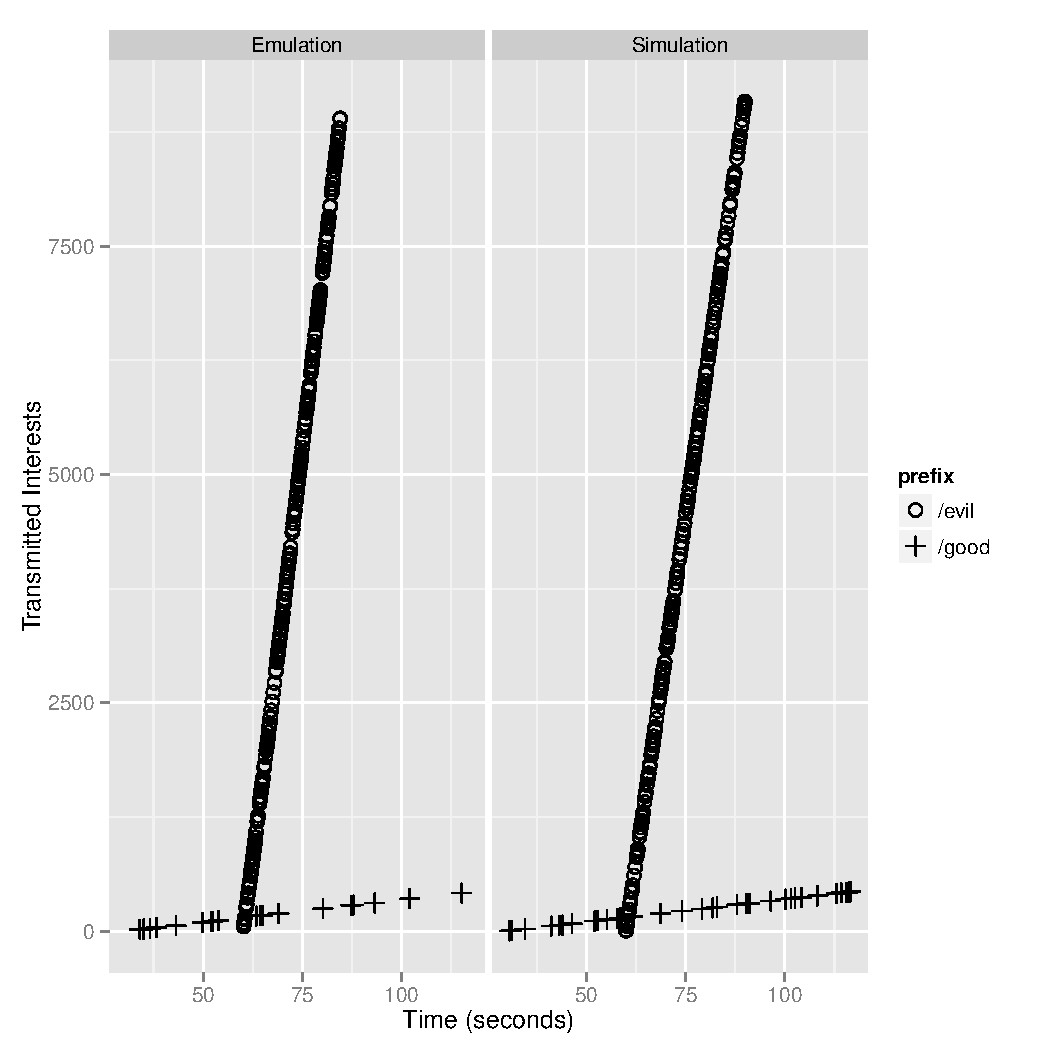
\includegraphics[scale=0.5]{figures/sim-emu-power.pdf}
%  \caption{Strength of Interest flooding attack}
%  \label{fig:simemupower}
%\end{figure}

%\begin{figure}[htpb]
%  \centering
%  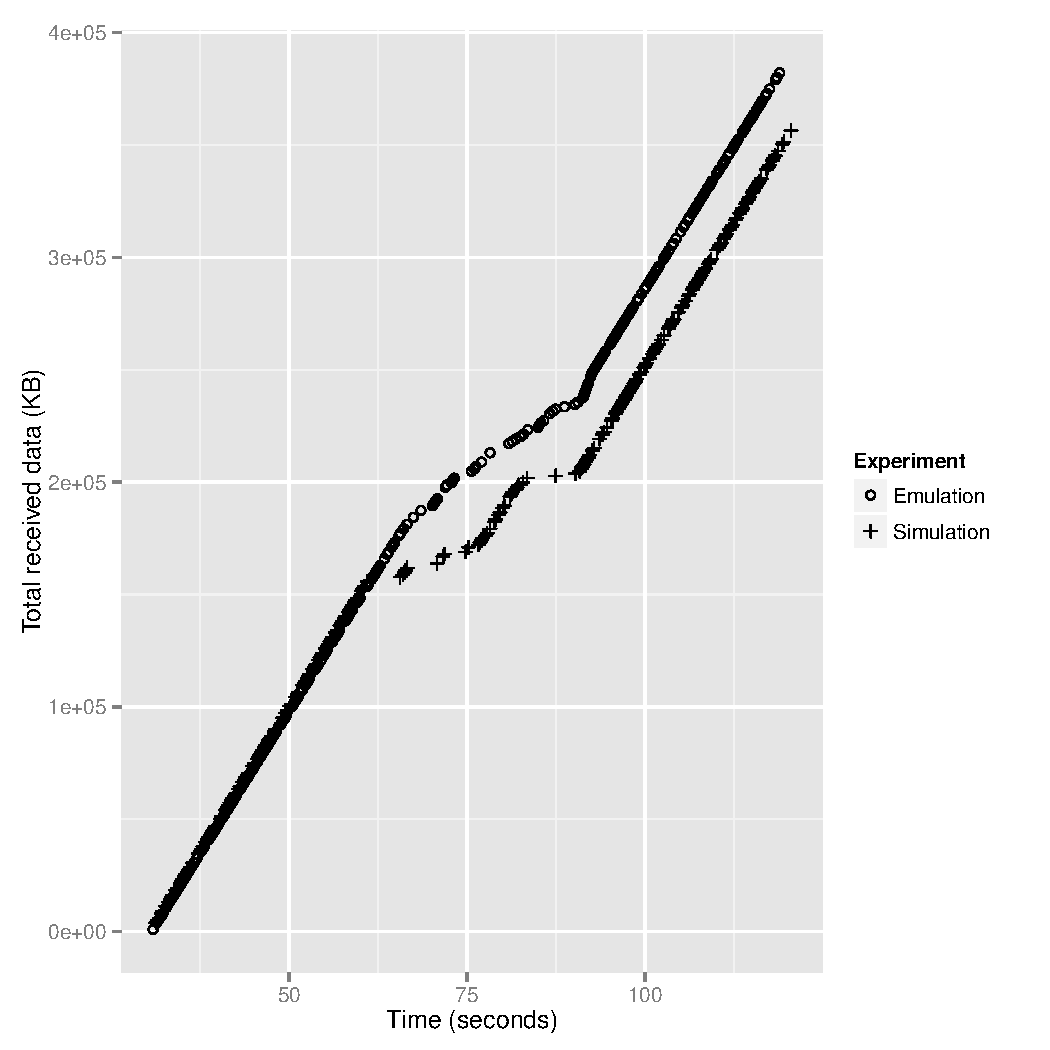
\includegraphics[scale=0.5]{figures/sim-emu-performance.pdf}
%  \caption{Data retrieval by legitimate clients}
%  \label{fig:simemuperf}
%\end{figure}


%%% Local Variables: 
%%% mode: latex
%%% TeX-master: "paper"
%%% End: 
